\section{Hydrostatik}
	
	\subsection{Druck}										%Druck
	\begin{table}[h!]

	\begin{tabular}{ | m{6cm} | m{6cm} | m{6cm} | }
	\hline
	Abbildung & Formeln & Einheiten \\ \hline
	\midrule
	\begin{minipage}{.1\textwidth}
	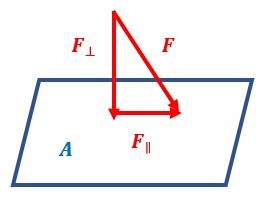
\includegraphics[width=5cm]{Figures/Druck.png}
	\end{minipage}
	&
	%\begin{minipage}[t]{5cm}
	\begin{itemize}
	\item $p=\frac{F_{\perp}}{A}$
	\item $\tau=\frac{F_{\parallel}}{A}$
	\item {\color{red}$\tau = 0 $ für ruhende Fluide} 
	\end{itemize}
	%\end{minipage}
	& 
	%\begin{minipage}{5cm}
	\begin{itemize}
	\item $p=[\frac{N}{m^2}]=Pa$
	\item $\tau=[\frac{N}{m^2}]=Pa$
	\item $\tau=Scherung$ 
	\end{itemize}
	%\end{minipage}
	\\ \hline
	\end{tabular}
	\end{table}

	\subsection{Schweredruck}							%Schweredruck
	\begin{table}[h!]

	\begin{tabular}{ | m{6cm} | m{6cm} | m{6cm} | }
	\hline
	Abbildungen & Formeln & Einheiten \\ \hline
	\midrule
	\begin{minipage}{.3\textwidth}
	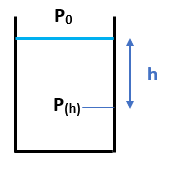
\includegraphics[width=4cm]{Figures/Schweredruck1.png}\\
	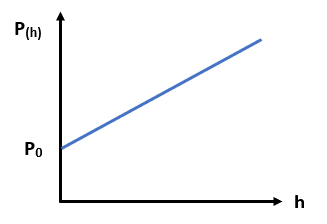
\includegraphics[width=4cm]{Figures/Schweredruck2.png}\\
	\end{minipage}
	&
	%\begin{minipage}[t]{5cm}
	\begin{itemize}
	\item $p_{(h)}=p_{0}+\rho*g*h$
	\item {\color{red}Wenn der Überdruck gefragt ist, dann ist ohne den Umgebungsdruck zu rechnen, also:}
	\item $p_{(h)}=\rho*g*h$
	\item Kraft auf eine Fläche (z.B. Fenster ) in der Tiefe: 
	\item $F=p*A$
	\item {\color{red}Als Höhe ist die Mitte der Fläche anzunehmen}
	\end{itemize}
	%\end{minipage}
	& 
	%\begin{minipage}{5cm}
	\begin{itemize}
	\item $p_{(h)},p_{0}=[\frac{N}{m^2}]=Pa$
	\item $p_{(h)}=$ Druck in der Tiefe
	\item $p_{0}=$ Umgebungsdruck 
	\item $p_{0}=101325 [Pa]$ 
	\item $\rho=[\frac{kg}{m^3}]$ 
	\item $g=9.81[\frac{m}{s^2}]$ 
	\item $h=[m]=$ Tiefe 
	\item $F=[N]$
	\item $A=[m^{2}]$
	
	\end{itemize}
	%\end{minipage}
	\\ \hline
	\end{tabular}
	\end{table}

	\subsection{Auftrieb: Prinzip des Archimedes}				%Auftrieb Prinzip des Archimedes
	\begin{table}[h!]
	\begin{tabular}{ | m{6cm} | m{7cm} | m{5cm} | }
	\hline
	Abbildung & Formeln & Einheiten \\ \hline
	\midrule
	\begin{minipage}{.3\textwidth}
	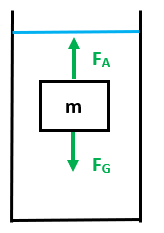
\includegraphics[width=3cm]{Figures/Auftrieb.png}
	\end{minipage}
	&
	%\begin{minipage}[t]{5cm}
	\begin{itemize}
	\item $F_{G}=Gewichtskraft$
	\item $F_{G}=\rho_{K}*V*g$
	\item $F_{A}=Auftriebskraft$
	\item $F_{A}=\rho_{F}*V*g$
	\item {\color{red}Wenn etwas oben auf schwimmt, herrscht keine Beschleunigung. Dann gilt: $F_{A}=F_{G}$}
	\item {\color{red}Als \textbf{Tiefgang} wird der Teil des Körpers bezeichnet der im Wasser ist. } 
	\end{itemize}

	%\end{minipage}
	& 
	%\begin{minipage}{5cm}
	\begin{itemize}
	\item $F_{A},F_{G}=[N]$
	\item $\rho_{K}=$ Dichte Körper
	\item $\rho_{F}=$ Dichte Flüssigkeit
	\item $\rho_{F},\rho_{K}=[\frac{kg}{m^{3}}]$
	\item $V=[m^{3}]$
	\item $g=9.81[\frac{m}{s^{2}}]$
	\end{itemize}
	%\end{minipage}
	\\ \hline
	\end{tabular}
	\end{table}

\newpage
\vspace*{-3cm}
\subsection{Druck und Überdruck}				%Überdruck
\begin{table}[h!]
	\begin{tabular}{ | m{6cm} | m{6cm} | m{6cm} | }
		\hline
		Abbildung & Formeln & Einheiten \\ \hline
		\midrule
		\begin{minipage}{.3\textwidth}
			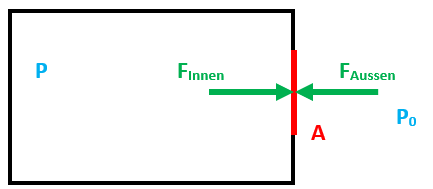
\includegraphics[width=4.5cm]{Figures/Ueberdruck}
		\end{minipage}
		&
		%\begin{minipage}[t]{5cm}
		\begin{itemize}
			\item $F=F_{I}-F_{A}=p*A-p_{0}*A$
			\item $A*(p-p_{0})=\Delta p*A$
			
			\item {\color{red}$\Delta p=$Überdruck} 
		\end{itemize}
		%\end{minipage}
		& 
		%\begin{minipage}{5cm}
		\begin{itemize}
			\item $p,p_{0},\Delta p=[\frac{N}{m^2}]=Pa$
			\item $F,F_{I},F_{A}=[N]$
			\item $A=[m^2]$ 
			\item $A=$Fläche der Scheibe 	
		\end{itemize}
		%\end{minipage}
		\\ \hline
	\end{tabular}
\end{table}

\subsection{Kompression}				%Kompression
\begin{table}[h!]
	\begin{tabular}{ | m{6cm} | m{6cm} | m{6cm} | }
		\hline
		Abbildung & Formeln & Einheiten \\ \hline
		\midrule
		\begin{minipage}{.3\textwidth}
			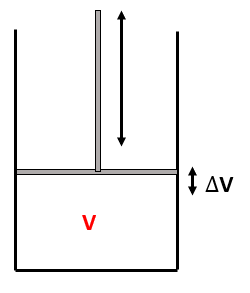
\includegraphics[width=4.5cm]{Figures/Kompression}
		\end{minipage}
		&
		%\begin{minipage}[t]{5cm}
		\begin{itemize}
			\item $\frac{\Delta V}{V}=-\kappa * \Delta p$
			\item $\kappa = -\dfrac{1}{V}*\dfrac{\Delta V}{\Delta p}$
			\item {\color{red}$K=\frac{1}{\kappa}$} 
			\item {\color{red}$K=$Kompressionsmodul}
		\end{itemize}
		%\end{minipage}
		& 
		%\begin{minipage}{5cm}
		\begin{itemize}
			\item $\Delta p=[\frac{N}{m^2}]=Pa$
			\item $\kappa =[\frac{1}{Pa}]$
			\item $V, \Delta V =[m^3]$ 		
		\end{itemize}
		%\end{minipage}
		\\ \hline
	\end{tabular}
\end{table}


\subsection{Barometrische Höhenformel}				%Barometrische Höhenformel
\begin{table}[h!]
	\begin{tabular}{ | m{6cm} | m{6cm} | m{6cm} | }
		\hline
		Abbildung & Formeln & Einheiten \\ \hline
		\midrule
		\begin{minipage}{.3\textwidth}
			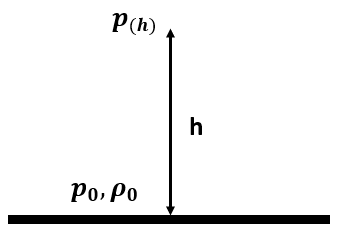
\includegraphics[width=4.5cm]{Figures/barometrisch}
		\end{minipage}
		&
		%\begin{minipage}[t]{5cm}
		\begin{itemize}
			\item $p_{(h)}=p_{0}*e^{-\dfrac{\rho_{0}*g*h}{p_{0}}}$
		\end{itemize}
		%\end{minipage}
		& 
		%\begin{minipage}{5cm}
		\begin{itemize}
			\item $p_{(h)}=[\frac{N}{m^2}]=Pa$
			\item $p_{0}=[\frac{N}{m^2}]=Pa$
			\item $\rho_{0}=[\frac{kg}{m^3}]$ 
			\item $g=[\frac{m}{s^2}]$ 	
			\item $h=[m]$ 				
		\end{itemize}
		%\end{minipage}
		\\ \hline
	\end{tabular}
\end{table}
	
	
\subsection{Oberflächenspannung}				%Oberflächenspannung
\begin{table}[h!]
	\begin{tabular}{ | m{6cm} | m{6cm} | m{6cm} | }
		\hline
		Abbildung & Formeln & Einheiten \\ \hline
		\midrule
		\begin{minipage}{.3\textwidth}
			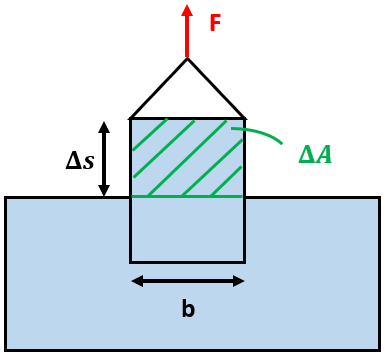
\includegraphics[width=4.5cm]{Figures/oberflaechenspannung}
		\end{minipage}
		&
		%\begin{minipage}[t]{5cm}
		\begin{itemize}
			\item $\sigma=\dfrac{\Delta W}{\Delta A}=\dfrac{\Delta W}{\Delta s * b * 2}$
			\item $\sigma=\dfrac{F}{2*b}$
			
		\end{itemize}
		%\end{minipage}
		& 
		%\begin{minipage}{5cm}
		\begin{itemize}
			\item $\sigma=[\frac{N}{m}]$
			\item $\sigma=$ Oberflächenspannung
			\item $\Delta W=[Ws]$
			\item $\Delta A=[m^2]$
		    \item $\Delta s,b=[m]$		
		\end{itemize}
		%\end{minipage}
		\\ \hline
	\end{tabular}
\end{table}

	{\color{red} Ideale Flüssigkeit $\implies$ reibungsfrei und inkompressibel} \\
	{\color{red}Ideales Gas $\implies$ Gesetz von Boyle-Mariotte $=p*V=constant\implies$ Gilt nur für konstante Temperatur T!} \\
	 Isotherm = Die Temperatur bleibt gleich (bzw. man lässt genug Zeit zum Temmperaturausgleich \\	
	 Adiabatisch = Ohne Wärmeaustausch mit der Umgebung\\
	 Barotrop = Die Dichte einer Flüssigkeit ist nur von Druck abhängig		\\

